% 09.tex
% Benjamin Davies
% 2017 05 12

\begin{enumerate}

	\item
	A consumer solves
	\[ \max_xu(x)\ \text{subject to}\ px\le w, \label{eq:1good_prob} \]
	where~$x$ denotes the demand for a single good with price~$p>0$ and~$w>0$ denotes the consumer's wealth.
	Assume that the utility function~$u(x)$ is strictly increasing and concave in~$x$.
	%
	\begin{enumerate}

		\item
		Show that the optimal solution~$x^*$ satisfies
		\[ u'(x^*)=\delta p, \label{eq:1good_foc} \]
		where~$\delta\ge0$ is the Lagrange multiplier for the budget constraint.
		%
		\begin{solution}
			The Lagrangian for~\eqref{eq:1good_prob} is given by
			\[ \Lcal(x,\delta)=u(x)+\delta(w-px). \]
			The optimal demand~$x^*$ satisfies the first-order condition
			%
			\begin{align}
				0
				&= \pder{\Lcal(x^*,\delta)}{x}\\
				&= u'(x^*)-\delta p,
			\end{align}
			%
			which can be rearranged for~\eqref{eq:1good_foc}.
		\end{solution}

		\item
		Show that~$x^*$ is (i)~increasing in~$w$ and (ii)~decreasing in~$p$.
		%
		\begin{solution}
			From~\eqref{eq:1good_foc} we have
			\[ \delta=\frac{u'(x^*)}{p}, \]
			which is strictly positive since~$u(x)$ is strictly increasing.
			Hence the budget constraint is binding and so
			\[ px^*=w. \]
			Differentiating with respect to~$w$ gives
			\[ p\pder{x^*}{w}=1 \]
			so that
			\[ \pder{x^*}{w}=\frac{1}{p} \]
			is strictly positive, while differentiating with respect to~$p$ gives
			\[ x^*+p\pder{x^*}{p}=0 \]
			so that
			\[ \pder{x^*}{p}=-\frac{x^*}{p} \]
			is strictly negative because~$x^*=w/p>0$.
			Hence~$x^*$ is increasing in~$w$ and decreasing in~$p$.
		\end{solution}

		\item
		Let~$v(p,w)=u(x^*)$ denote the consumer's indirect utility function.
		Show that~$v(p,w)$ is (i)~increasing in~$w$ and (ii)~decreasing in~$p$.
		%
		\begin{solution}
			Differentiating~$v(p,w)$ with respect to~$w$ gives
			%
			\begin{align}
				\pder{v(p,w)}{w}
				&= u'(x^*)\pder{x^*}{w}\\
				&= \frac{u'(x^*)}{p}\\
				&= \delta,
			\end{align}
			%
			which is strictly positive.
			Hence~$v(p,w)$ is increasing in~$w$.
			Similarly, differentiating~$v(p,w)$ with respect to~$p$ gives
			%
			\begin{align}
				\pder{v(p,w)}{p}
				&= u'(x^*)\pder{x^*}{p}\\
				&= -\frac{u'(x^*)x^*}{p}
			\end{align}
			%
			which is strictly negative.
			Hence~$v(p,w)$ is decreasing in~$p$.
		\end{solution}

	\end{enumerate}

	\item
	A consumer with initial wealth~$w_0$ and utility function~$u(w)=\ln(w)$ is exposed to a risk that will decrease his wealth by an amount~$x\in(0,w_0)$ with probability~$p$ or increase his wealth by~$x$ with probability~$(1-p)$.
	%
	\begin{enumerate}

		\item
		Write down an expression for the consumer's expected utility.
		%
		\begin{solution}
			The consumer has expected utility
			\[ \E[u(w)]=p\ln(w_0-x)+(1-p)\ln(w_0+x). \]
		\end{solution}

		\item
		Suppose that~$\phi$ satisfies the indifference condition
		\[ \E[u(w)]=u(w_0-\phi). \label{eq:risk_aversion_indiff}\]
		Use Jensen's inequality to show that~$\phi>(2p-1)x$.
		%
		\begin{solution}
			Recall that~$\ln(t)$ is strictly concave in~$t$.
			Hence, by Jensen's inequality, we have
			%
			\begin{align}
				\E[u(w)]
				&= p\ln(w_0-x)+(1-p)\ln(w_0+x)\\
				&< \ln(p(w_0-x)+(1-p)(w_0+x))\\
				&= \ln(w_0+(1-2p)x)
			\end{align}
			%
			so that
			\[ \ln(w_0-\phi)<\ln(w_0+(1-2p)x). \]
			But~$\ln(t)$ is strictly increasing in~$t$ and therefore
			\[ w_0-\phi<w_0+(1-2p)x \]
			from which it follows that~$\phi>(2p-1)x$.
		\end{solution}

		\item
		Let~$p=0.5$.
		Show graphically that~$\phi<x$.
		\vskip\baselineskip

		\emph{Hint}: sketch the consumer's utility function~$u(w)=\ln(w)$ in~$\R^2$ and label the points~$(w_0-x,u(w_0-x))$, $(w_0,u(w_0))$, etc., and compare the positions of~$w_0-x$ and~$w_0-\phi$.
		%
		\begin{solution}
			The consumer's prospects can be shown graphically as follows.
			%
			\begin{center}
				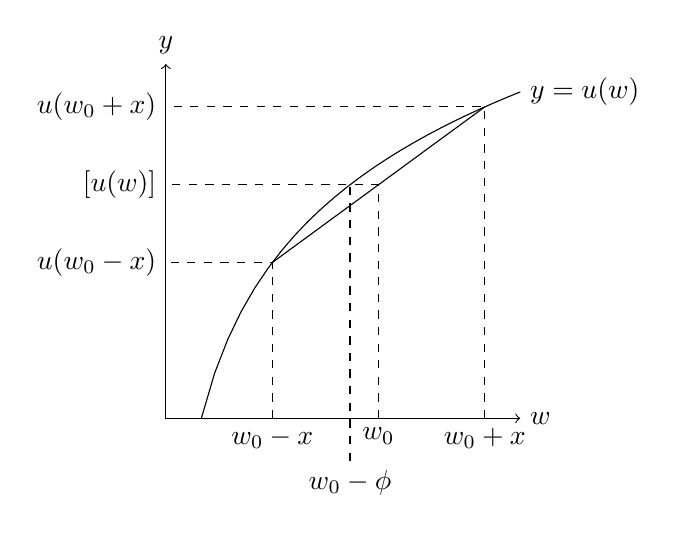
\begin{tikzpicture}[xscale=0.45, yscale=1.8]

					% axes
					\draw [<->] (10,0) node [right] {$w$} -- (0,0) -- (0,2.5) node [above] {$y$};

					% utility curve
					\draw [domain=1:10] plot (\x, {ln(\x)}) node [right] {$y=u(w)$};

					% labels
					\draw [dashed] (3,0) node [below] {$w_0-x$} -- (3,1.0986) -- (0,1.0986) node [left] {$u(w_0-x)$};
					\draw [dashed] (9,0) node [below] {$w_0+x$} -- (9,2.1972) -- (0,2.1972) node [left] {$u(w_0+x)$};
					\draw (3,1.0986) -- (9,2.1972);
					\draw [dashed] (6,0) node [below] {$w_0$} -- (6,1.6479) -- (0,1.6479) node [left] {$\E[u(w)]$};
					\draw [dashed] (5.1960,-0.3) node [below] {$w_0-\phi$} -- (5.1960,1.6479);

				\end{tikzpicture}
			\end{center}
			%
			The consumer's expected utility~$\E[u(w)]$ lies at the midpoint of the chord between the points~$(w_0-x,u(w_0-x))$ and~$(w_0+x,u(w_0+x))$ because~$p=0.5$.
			The level of wealth~$w_0-\phi$ satisfying~\eqref{eq:risk_aversion_indiff} is shown.
			Clearly~$w_0-x<w_0-\phi$ and therefore~$\phi<x$ as required.

		\end{solution}

	\end{enumerate}

\end{enumerate}
